\chapter{SCL: Training-Free Self-Calibrating Control Layer}\label{ch:scl}

\section{Introduction}\label{sec:scl-intro}
Multi-object trackers rely on score thresholds tuned for one detector. When the detector is replaced, retrained, or compressed, its scores shift, and the tuned thresholds silently stop fitting. AC-MOT, the controller of Chapter~\ref{ch:acmot}, adapts the detector to the scene but keeps the tracker's thresholds and assumes that the detector's scores have the scale for which they were tuned. This chapter removes that assumption. It presents the second controller of the thesis, a training-free self-calibrating control layer (SCL) between an unchanged detector and an unchanged tracker. The chapter is based on the manuscript submitted to The Visual Computer \cite{ismail2026scl}.

SCL splits the logits of recent scores twice with Otsu's method and classifies the stream as clean or noisy, without labels or future frames. Its novelty is selective, host-aware adaptation. On clean streams it keeps the tracker's scores and lowers a threshold only if it would reject the confident detections; on noisy streams it selects and rescores the detections and sets the thresholds. It acts through four published tracker settings and passes on weak detections that continue tracks, so one frozen configuration serves single-stage and two-stage trackers.

The layer was evaluated on seven trackers, four detection sources, and three datasets, and all changes below are relative to the tracker alone. When the detector scores were halved, two trackers fell to zero HOTA; with SCL both recovered at least 97\% of it. With a replacement detector, RT-DETR-L, SCL raised the MOTA of ByteTrack and BoT-SORT by 12.6\% and 16.3\% and cut their identity switches by 43\% and 47\%, respectively. It also raised the HOTA of PD-SORT, a tracker not seen during design, by 0.9\%, and it kept four well-matched trackers within 0.1\% of their own accuracy. SCL adds on average no more than 2.95 ms per frame on an ordinary processor, so a detector can be replaced or retrained without retuning the tracker.

Section~\ref{sec:scl-setting} states the problem and the requirements of the layer. Section~\ref{sec:scl} presents the five steps of SCL, its host contract, and its fixed values. Section~\ref{sec:scl-dev} describes how it was developed and frozen. Section~\ref{sec:scl-setup} gives the experimental setup, Section~\ref{sec:scl-results} the results on MOT17, KITTI, and UAVDT, Section~\ref{sec:scl-compare} the comparison with adaptive-threshold methods, Section~\ref{sec:scl-ablation} the ablation and sensitivity analysis, and Section~\ref{sec:scl-runtime} the runtime. Section~\ref{sec:scl-discussion} discusses the results, and Section~\ref{sec:scl-summary} summarizes the chapter.

\section{Problem Setting and Requirements}\label{sec:scl-setting}
In this chapter the tracker that SCL serves is called the \emph{host}. A host reads detector scores through its published thresholds (Section~\ref{sec:bg-confidence}): a score $a$ needed to match a track, a score $b$ needed to start one, and the lowest score $\ell$ it uses at all. These values were tuned for one detector. The detector and the host are \emph{compatible} when the confident detections of the objects pass the host's thresholds and the background clutter does not. Compatibility is a property of the pair, not of either component: the same tracker can be compatible with one detector and incompatible with another, and the same detector can serve one tracker well and another badly.

When compatibility is lost, single-stage and two-stage hosts fail in different ways. A single-stage host ignores every box below one threshold, so a lower score scale removes most of its boxes and it has no step that could continue a track through a weak detection. A two-stage host keeps continuing tracks through its low-score step, but it may stop starting new tracks, as in the example of ByteTrack with halved scores (Section~\ref{sec:intro-motivation}). A noisy detector, in turn, can pass many false positives above the host's thresholds, as RT-DETR-L did on the UAVDT test split (Section~\ref{sec:scl-res-uavdt}).

The problem is to restore compatibility online, frame by frame, without changing either component. The layer must meet six requirements:
\begin{enumerate}
\item \emph{Label-free:} it decides from the detector scores alone, without ground truth or a calibration set.
\item \emph{Causal:} the decision for frame $t$ uses only the scores of earlier frames, the current candidates, and the tracks of the previous frame.
\item \emph{Training-free and external:} the detector and the host are frozen; their code, weights, and association are unchanged, and only the values of the host's thresholds and its input are set for each frame.
\item \emph{Selective:} a well-matched pair must keep its own output, because an adaptation that always acts can lower the accuracy of strong trackers (Section~\ref{sec:scl-prior}).
\item \emph{Host-aware and tracker-agnostic:} the same rules must serve single-stage and two-stage hosts, through values that each tracker already publishes.
\item \emph{Inexpensive:} the layer must run on an ordinary processor in a few milliseconds per frame.
\end{enumerate}

\section{The SCL Framework}\label{sec:scl}
SCL is a lightweight, rule-based layer operating between a frozen detector and a frozen host without modifying their underlying algorithms. The host gives SCL four of its published settings, the host contract (Section~\ref{sec:scl-contract}), and SCL returns, for every frame, the candidates, scores, thresholds, and matching tolerance with which the host runs its own update.

\subsection{Overview}\label{sec:scl-overview}
Figure~\ref{fig:scl-arch} illustrates the five processing steps of SCL for frame $t$. First, Otsu-based logit partitioning (Step~1) divides recent detection scores into background, uncertain, and confident groups. Next, detection stream classification (Step~2) determines whether the score distribution is clean or noisy based on historical confidence statistics. Mode-adaptive candidate selection (Step~3) then retains, removes, or remaps detection scores and adjusts the tracker's confidence thresholds according to the operating mode. Track-guided weak detection recovery (Step~4) allows eligible low-confidence detections to support track continuity. Finally, camera motion-adaptive matching tolerance (Step~5) adjusts the association criterion according to estimated camera motion. The host contract provides the tracker's published parameters, while the tracker performs its original association and track-management operations unchanged.

\begin{figure}[tbp]
\centering
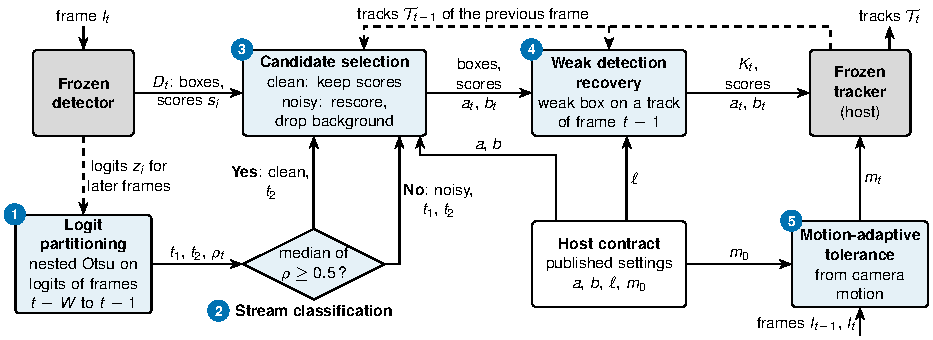
\includegraphics[width=0.98\textwidth]{figures/scl_architecture_v3.pdf}
\caption{SCL between a frozen detector and a frozen tracker (the host), for frame $t$. Arrows are labelled with the data they carry; dashed arrows carry data from earlier frames. The diamond (Step 2) is a decision: clean (Yes) if the median of $\rho$ is at least 0.5, noisy (No) otherwise. Steps 1--5: Sections~\ref{sec:scl-calib}--\ref{sec:scl-motion}; host contract: Section~\ref{sec:scl-contract}; symbols: Table~\ref{tab:scl-symbols}.}
\label{fig:scl-arch}
\end{figure}

Table~\ref{tab:scl-symbols} lists every symbol in plain words, with its value in the clean stream of Fig.~\ref{fig:scl-groups}a, which the subsections below follow from input to output.

\begin{table}[tbp]
\centering
\caption{The symbols of SCL in plain words. Example: the value in the clean stream of Fig.~\ref{fig:scl-groups}a (MOT17-02, frame 101, ByteTrack in its official setting), as recorded by the frozen SCL; e.g.: a worked example from the text.}
\label{tab:scl-symbols}
\begin{tabular}{l>{\raggedright\arraybackslash}p{7.6cm}>{\raggedright\arraybackslash}p{3.8cm}}
\toprule
Symbol & Meaning & Example\\
\midrule
$s_i$, $z_i$ & detector score of candidate $i$, between 0 and 1, and its logit, Eq.~\eqref{eq:scl-logit} & e.g.\ 0.9 and $\log 9=2.2$\\
$W$, $Z_t^W$ & number of past frames whose logits are pooled; the logits of frames $t-W$ to $t-1$ & 10; 916 logits\\
$t_1$, $t_2$ & first split (background lies below it); second split (confident lies above it) & $-0.78$ (0.32); 0.95 (0.72)\\
$\rho_t$ & share of confident candidates in the foreground, Eq.~\eqref{eq:scl-rho} & $175/263=0.67$\\
median $\rho$ & median of $\rho$ over the stream so far; clean if $\ge0.5$ & 0.63: clean\\
$a$, $b$, $\ell$ & the tracker's published scores to match a track and to start one, and the lowest score it uses & 0.6, 0.7, 0.1\\
$m_0$ & the tracker's matching tolerance: 1 minus the smallest IoU that matches & 0.8 (IoU $\ge0.2$)\\
$a_t$, $b_t$, $m_t$ & the thresholds and tolerance SCL passes for frame $t$, Eqs.~\eqref{eq:scl-clean} and~\eqref{eq:scl-motion} & 0.6, 0.7 (kept); 0.8\\
$u_i$, $\tilde{s}_i$ & rank of $s_i$ among stored scores; the new score of the noisy mode, Eq.~\eqref{eq:scl-remap} & e.g.\ $u_i=0.8\to\tilde{s}_i=0.9$\\
$\mathcal{T}_{t-1}$, $K_t$ & the tracks of the previous frame; the candidates passed to the tracker & --\\
$g_t$, $r_t$ & camera shift between two frames; its ratio to the usual shift & e.g.\ $r_t=2$\\
\bottomrule
\end{tabular}
\end{table}

\subsection{Inputs and Outputs}\label{sec:scl-problem}
In each frame $t$, the detector gives candidates $D_t=\{(\mathbf{x}_i,s_i,c_i)\}$, each with a box $\mathbf{x}_i$, a score $s_i\in(0,1)$, and a class $c_i$. The layer works on the logit of each score (Eq.~\eqref{eq:bg-logit}),
\begin{equation}
z_i=\log\frac{s_i}{1-s_i},
\label{eq:scl-logit}
\end{equation}
so that 0.5 gives $z_i=0$, 0.9 gives $\log 9=2.2$, and 0.1 gives $-2.2$. Because the logit spreads out the regions near 0 and 1, where detector scores crowd, the splits of Step~1 separate the groups more clearly, and a change of temperature, which divides all logits by the same number, is a simple stretch that the splits follow.

The host gives its contract $h=(a,b,\ell,m_0)$: the score $a$ needed to match a track, the score $b$ needed to start one, the lowest score $\ell$ it uses, and its matching tolerance $m_0$, one minus the smallest intersection over union (IoU) that counts as a match. A single-stage tracker has $\ell=\min(a,b)$, a two-stage tracker $\ell<\min(a,b)$. For ByteTrack in its official setting, $a=0.6$, $b=0.7$, $\ell=0.1$, and $m_0=0.8$ (Table~\ref{tab:scl-contracts}). In every frame the layer returns
\begin{equation}
\left(K_t,\tilde{s},a_t,b_t,m_t\right)=
\mathcal{L}\left(Z_{<t},D_t,\mathcal{T}_{t-1},g_t;\,h\right):
\label{eq:scl-layer}
\end{equation}
the candidates $K_t$, their scores, and the thresholds and tolerance for the tracker, from the logits $Z_{<t}$ of earlier frames, the tracks $\mathcal{T}_{t-1}$, and the camera motion $g_t$ between frames $I_{t-1}$ and $I_t$; no future frame is used.

\begin{table}[tbp]
\centering
\caption{Host contracts: the four published settings $(a,b,\ell,m_0)$ of each tracker that SCL reads (Section~\ref{sec:scl-problem}), and where each value comes from; $\theta$: the published IoU threshold, $m_0=1-\theta$.}
\label{tab:scl-contracts}
\begin{tabular}{>{\raggedright\arraybackslash}p{2.6cm}>{\raggedright\arraybackslash}p{1.6cm}cccc>{\raggedright\arraybackslash}p{5.6cm}}
\toprule
Tracker (setting) & Type & $a$ & $b$ & $\ell$ & $m_0$ & Published settings behind the values\\
\midrule
ByteTrack (official) & two-stage & 0.6 & 0.7 & 0.1 & 0.8 & track\_thresh 0.6; new tracks $+$0.1; second step from 0.1; match\_thresh 0.8\\
ByteTrack (library) & two-stage & 0.25 & 0.25 & 0.1 & 0.8 & Ultralytics bytetrack.yaml: high 0.25, new 0.25, low 0.1, match 0.8\\
BoT-SORT (library) & two-stage & 0.25 & 0.25 & 0.1 & 0.8 & Ultralytics botsort.yaml: the same four values\\
SparseTrack & two-stage & 0.6 & 0.7 & 0.1 & 0.85 & track\_thresh 0.6; new tracks $+$0.1; second step from 0.1; match\_thresh 0.85\\
BoostTrack & two-stage & 0.6 & 0.6 & 0.1 & 0.7 & det\_thresh 0.6; every detection from 0.1 can be boosted; $\theta=0.3$\\
Hybrid-SORT & two-stage & 0.6 & 0.6 & 0.1 & 0.75 & det\_thresh 0.6; low-score step from 0.1; $\theta=0.25$\\
OC-SORT & single-stage & 0.6 & 0.6 & 0.6 & 0.7 & det\_thresh 0.6, no low-score step; $\theta=0.3$\\
PD-SORT & single-stage & 0.6 & 0.6 & 0.6 & 0.7 & det\_thresh 0.6, no low-score step; $\theta=0.3$\\
\bottomrule
\end{tabular}
\end{table}

\subsection{Otsu-Based Logit Partitioning and Confidence Estimation}\label{sec:scl-calib}
\emph{Step 1 in Fig.~\ref{fig:scl-arch}. Input:} the logits $Z_t^W$ of the candidates of the last $W=10$ frames. \emph{Output:} the splits $t_1$, $t_2$ and the confident share $\rho_t$.

The logits are split twice with Otsu's method \cite{goh2018otsu} (Eq.~\eqref{eq:bg-otsu}), which picks from the data alone the threshold that best separates two groups: $t_1$ separates background (low logits) from foreground, and $t_2$, found on the foreground only, divides it into uncertain and confident candidates. Otsu's method is used because it picks a split without labels or tuning, and applying it twice gives the three groups that one threshold cannot. The share of confident candidates in the foreground,
\begin{equation}
\rho_t=\frac{\left|\{z\in Z_t^W: z\ge t_2\}\right|}{\left|\{z\in Z_t^W: z\ge t_1\}\right|},
\label{eq:scl-rho}
\end{equation}
describes the shape of the score distribution and needs no labels. For example, for the scores 0.02, 0.03, 0.05, 0.4, 0.5, 0.9, and 0.95, the splits fall at $t_1=-1.67$ (score 0.16) and $t_2=1.10$ (score 0.75): three scores are background, two uncertain, and two confident, so $\rho_t=2/4=0.5$. In the clean stream of Fig.~\ref{fig:scl-groups}a, the window holds 916 candidates: 653 below $t_1=-0.78$ (score 0.32), 88 between the splits, and 175 above $t_2=0.95$ (score 0.72), so $\rho_t=175/(88+175)=0.67$; in the noisy stream of Fig.~\ref{fig:scl-groups}b, 1,037 are background, 99 uncertain, and 83 confident, so $\rho_t=83/(99+83)=0.46$. As clutter usually gives more candidates than objects do, a window with fewer candidates below $t_1$ than above it counts as clean, $\rho_t=1$ (background check), which does not apply in Fig.~\ref{fig:scl-groups}.

\begin{figure}[tbp]
\centering
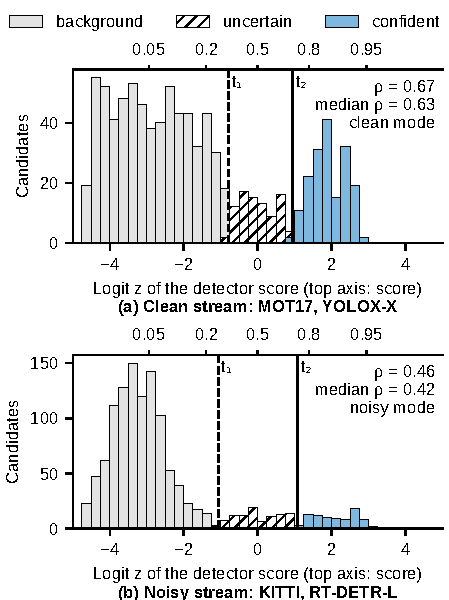
\includegraphics[width=0.62\textwidth]{figures/scl_score_groups_v3.pdf}
\caption{What SCL sees before its decision for frame 101: the logits of the candidates of the last 10 frames (top axis: the same position as a score). Dashed line: $t_1$; solid line: $t_2$; light gray: background; hatched: uncertain; blue: confident. (a) MOT17 sequence MOT17-02, YOLOX-X, ByteTrack (official): median $\rho=0.63\ge0.5$, clean. (b) KITTI sequence 0001, RT-DETR-L, ByteTrack (library): median $\rho=0.42<0.5$, noisy. Values recorded by the frozen SCL.}
\label{fig:scl-groups}
\end{figure}

\subsection{Median-Based Detection Stream Classification}\label{sec:scl-regimes}
\emph{Step 2 in Fig.~\ref{fig:scl-arch}. Input:} the values $\rho$ of all frames so far. \emph{Output:} the mode of frame $t$.

The mode describes the distribution of the scores, not whether a single detection is correct: the stream is clean at frame $t$ if the median of all $\rho$ values so far is at least one half, a majority rule, and noisy otherwise; before the first valid split it is cold. In Fig.~\ref{fig:scl-groups}a, frames 2 to 101 give a median of 0.63, so frame 101 is clean; in Fig.~\ref{fig:scl-groups}b the median is 0.42, so it is noisy. The whole-stream median keeps the mode stable against a few frames of blur or occlusion, and during development this rule raised the HOTA of ByteTrack and OC-SORT (Section~\ref{sec:scl-steps}), while the groups, and in the clean mode the thresholds of Step~3, follow a new score scale within $W$ frames.

\subsection{Mode-Adaptive Detection Candidate Selection and Threshold Adjustment}\label{sec:scl-modes}
\emph{Step 3 in Fig.~\ref{fig:scl-arch}. Input:} $D_t$, the mode, $t_1$, $t_2$, the thresholds $a$, $b$, and the tracks $\mathcal{T}_{t-1}$. \emph{Output:} the kept boxes, their scores, and the thresholds $a_t$, $b_t$.

\emph{Cold and clean modes.} The tracker keeps its own scores, and only cross-class duplicates are removed. In the clean mode, a threshold that would reject the confident group is lowered to the score $\sigma(t_2)$ at which that group begins:
\begin{equation}
a_t=\min\!\left(a,\sigma(t_2)\right),\qquad b_t=\min\!\left(b,\sigma(t_2)\right).
\label{eq:scl-clean}
\end{equation}
In Fig.~\ref{fig:scl-groups}a, $\sigma(t_2)=0.72$ is above both $a=0.6$ and $b=0.7$, so the published thresholds are kept and the output equals that of the host alone, as for BoostTrack, ByteTrack at floor 0.1, and Hybrid-SORT on MOT17 (Section~\ref{sec:scl-res-mot17}). When the scores are halved, no score is above 0.5 and ByteTrack in its official setting never starts a track; $\sigma(t_2)$ falls with the scores below 0.5, Eq.~\eqref{eq:scl-clean} lowers both thresholds to it, and the confident candidates reach the tracker again.

\emph{Noisy mode.} Background candidates ($z<t_1$) are dropped. Each remaining score is replaced by its mid-rank $u_i\in(0,1)$ among the scores of a remap memory, which stores the scores kept in the first frame and in every 10th frame, the last 20 of them (equal scores count half):
\begin{equation}
\tilde{s}_i=
\begin{cases}
0.5+0.5\,u_i, & z_i\ge t_2,\\
0.1+0.4\,u_i, & t_1\le z_i<t_2,
\end{cases}
\label{eq:scl-remap}
\end{equation}
and both thresholds are set to $a_t=b_t=0.5$. A confident candidate with $u_i=0.8$ gets $0.5+0.5\cdot0.8=0.9$ and may start and continue tracks; an uncertain one with $u_i=0.3$ gets $0.1+0.4\cdot0.3=0.22$ and may only continue tracks through a tracker's low-score step. A weaker candidate that overlaps a stronger one with IoU above one half is removed, unless a different track of the previous frame claims it, which keeps people who stand close together in a crowd.

\emph{Score remapping is not probability calibration.} Calibration learns from labelled data the probability that a detection is correct \cite{kuppers2020detcalib}. The remap needs no labels: it keeps the order of the scores within each group and places the groups in fixed ranges, so that the tracker's own thresholds read the layer's decision (above 0.5: ``may start a track''; 0.1 to 0.5: ``may only continue one''), and it is unchanged by any order-preserving change of the scores.

\subsection{Track-Guided Weak Detection Recovery}\label{sec:scl-rescue}
\emph{Step 4 in Fig.~\ref{fig:scl-arch}. Input:} the output of Step~3, the tracks $\mathcal{T}_{t-1}$, and $\ell$. \emph{Output:} $K_t$, their scores, and $a_t$, $b_t$ for the tracker.

A track can be lost when its object gets low scores for a few frames, above all in a single-stage tracker, which has no low-score step. The rescue passes such a candidate, with its score raised just above the lowest threshold of the frame ($\ell$ for a two-stage tracker, the lower of $a_t$ and $b_t$ for a single-stage one), when it is in the foreground (or, for a single-stage tracker, when there is no background group), overlaps a track of the previous frame with IoU of at least one half, no other usable candidate covers that track, and the tracker could not see it otherwise. For ByteTrack in its official setting, a rescued candidate gets $0.101$ and enters its low-score step; for OC-SORT in a noisy frame it gets $0.501$. The rescue thus gives single-stage trackers the continuation step they lack, and the tracker itself still decides, with its own matching, whether and to which track the box is assigned.

\subsection{Camera Motion-Adaptive Matching Tolerance}\label{sec:scl-motion}
\emph{Step 5 in Fig.~\ref{fig:scl-arch}. Input:} the frames $I_{t-1}$, $I_t$ and the tolerance $m_0$. \emph{Output:} the tolerance $m_t$ of frame $t$.

In noisy frames, the matching tolerance grows with camera motion, which moves boxes far from their tracks; otherwise $m_t=m_0$. The motion $g_t$ is the shift between consecutive grayscale frames at quarter resolution, found by phase correlation \cite{tong2019fourier}, and $r_t$ is its ratio to its median over the last 100 frames ($r_t=1$ during a warm-up of 5 frames or if this median is zero):
\begin{equation}
m_t=\min\!\left(0.95,\;1-\frac{1-m_0}{\max(1,r_t)}\right).
\label{eq:scl-motion}
\end{equation}
With $m_0=0.8$, a match needs an IoU of at least 0.2; if the camera moves twice as much as usual ($r_t=2$), then $m_t=\min(0.95,\,1-0.2/2)=0.9$, and an IoU of 0.1 is enough. The cap 0.95 keeps a smallest overlap of 0.05.

\subsection{SCL Integration with Existing Trackers}\label{sec:scl-contract}
Each contract value in Table~\ref{tab:scl-contracts} comes from the tracker's published configuration; none is fitted. For each tracker family, a small adapter writes the layer's candidates, scores, thresholds, and tolerance into the tracker's existing parameters before each update and then calls the tracker's own update. The matching steps, motion model, track management, and any post-processing of the authors run unchanged, so the host stays frozen: its code, weights, and association algorithm do not change, only the values of its thresholds are set for each frame, and the rules are the same for every tracker.

\subsection{Fixed SCL Parameters}\label{sec:scl-constants}
Table~\ref{tab:scl-constants} lists all values of SCL. They were fixed before the external evaluation, are the same for every tracker, detector, and dataset, and none was chosen by searching over a range of values: they are standard values (the IoU of 0.5 of MOT evaluation and the common thresholds 0.5 and 0.1), definitions, or design choices kept fixed in all development stages. Algorithm~\ref{alg:scl-layer} gives Steps 1--5 for one frame.

\begin{table}[tbp]
\centering
\caption{The fixed values of SCL, their settings, and their sources; the same values are used for every tracker, detector, and dataset.}
\label{tab:scl-constants}
\begin{tabular}{>{\raggedright\arraybackslash}p{4.0cm}>{\raggedright\arraybackslash}p{5.4cm}>{\raggedright\arraybackslash}p{4.4cm}}
\toprule
Value & Setting & Source\\
\midrule
Window $W$ & 10 frames & design choice\\
Mode rule & clean if median $\rho\ge0.5$ & majority rule\\
Background check & $\rho=1$ if fewer below $t_1$ than above & rule: no background group\\
Noisy score ranges & $[0.5,1)$, $[0.1,0.5)$ & common thresholds\\
Noisy $a_t$, $b_t$ & 0.5 & common threshold\\
Remap memory & 20 frames, one every 10 & design choice\\
Duplicate, rescue IoU & 0.5 & MOT evaluation IoU\\
Rescued score & lowest threshold $+\,0.001$ & just above the threshold\\
Motion cue & phase correlation, quarter resolution & standard method \cite{tong2019fourier}\\
Motion history & 100 frames, warm-up 5 & design choice\\
Tolerance cap & 0.95 & minimum overlap 0.05\\
\bottomrule
\end{tabular}
\end{table}

\begin{algorithm}[tbp]
\caption{SCL for frame $t$; the comments name the steps of Fig.~\ref{fig:scl-arch}. The window holds the logits of frames $t-W$ to $t-1$, so the decision for frame $t$ uses no future frame.}\label{alg:scl-layer}
\begin{algorithmic}[1]
\Require candidates $D_t$, tracks $\mathcal{T}_{t-1}$, motion cue $g_t$, contract $(a,b,\ell,m_0)$, constants of Table~\ref{tab:scl-constants}
\Ensure candidates $K_t$, scores $\tilde{s}$, thresholds $a_t,b_t$, tolerance $m_t$
\State $z_i\gets$ logit of $s_i$ for all $i$ \Comment{Eq.~\eqref{eq:scl-logit}}
\If{no valid split exists} \Comment{e.g., first frame}
  \State mode $\gets$ cold; $(a_t,b_t)\gets(a,b)$
\Else
  \State $(t_1,t_2)\gets$ nested Otsu on the window \Comment{Step 1}
  \State $\rho_t\gets$ Eq.~\eqref{eq:scl-rho} with the background check
  \State mode $\gets$ clean if $\mathrm{median}(\rho)\ge0.5$, else noisy \Comment{Step 2}
\EndIf
\If{mode is cold or clean} \Comment{Step 3}
  \State remove cross-class duplicates; keep raw scores
  \If{clean} set $(a_t,b_t)$ by Eq.~\eqref{eq:scl-clean}
  \EndIf
\Else \Comment{noisy mode}
  \State remove duplicates with track context
  \State drop $z<t_1$; remap scores by Eq.~\eqref{eq:scl-remap}
  \State $a_t\gets0.5$; $b_t\gets0.5$
\EndIf
\State rescue continuations (not cold) \Comment{Step 4}
\State $m_t\gets$ Eq.~\eqref{eq:scl-motion} if noisy, else $m_0$ \Comment{Step 5}
\State pass $K_t$, $\tilde{s}$, $a_t$, $b_t$, $m_t$ to the tracker
\State add the logits left after duplicate removal to the window
\State add $g_t$ to the motion history
\State store the tracks of frame $t$ after the tracker update
\end{algorithmic}
\end{algorithm}

\section{Development and Freezing of SCL}\label{sec:scl-dev}
SCL was developed in three stages on development data: MOT17 with four trackers, KITTI, and the score transforms of Section~\ref{sec:scl-setup}. Section~\ref{sec:scl-prior} introduces the initial always-on banding (AOB) design and its limitations (Table~\ref{tab:scl-prior}). Section~\ref{sec:scl-steps} describes the incremental improvements that addressed these limitations, supported by the experimental comparisons in Table~\ref{tab:scl-ablation}. Finally, Section~\ref{sec:scl-freeze} explains the configuration freezing and validation performed before external evaluation, to ensure reproducibility and prevent changes based on later results.

\subsection{Initial Design and Limitations}\label{sec:scl-prior}
The earlier design AOB computed the same nested Otsu groups but treated every stream as noisy: in every frame it applied the groups, removed every weaker candidate that overlapped a stronger one with IoU above one half, and rescored all candidates by rank. On strong MOT17 trackers (Table~\ref{tab:scl-prior}), AOB lowered HOTA by 4.15 to 5.89 points, as the overlap rule deleted people hidden behind others in crowds and its thresholds were stricter than the trackers' own; with the same trackers, SCL changed HOTA by $+0.06$ for SparseTrack and left BoostTrack, online and with its gap-filling post-processing (GBI), identical to the host. The next steps therefore let the layer decide from the scores whether to act at all.

\begin{table}[tbp]
\centering
\caption{MOT17 val-half, published YOLOX-X detections: the earlier design AOB and the final SCL, each added to the same strong tracker (Host). Change: the run with the layer minus Host, for AOB with its 95\% paired-bootstrap interval (10,000 resamples, seed 42); bold: the interval does not include zero (a reliable change).}
\label{tab:scl-prior}
\begin{tabular}{lrrlrl}
\toprule
Metric & Host & Host+AOB & AOB change [95\% CI] & Host+SCL & SCL change\\
\midrule
\multicolumn{6}{l}{\textit{SparseTrack} \cite{liu2025sparsetrack}}\\
\quad HOTA & 68.88 & 64.72 & \textbf{$-4.15$ [$-5.54$, $-1.66$]} & 68.93 & $+0.06$\\
\quad MOTA & 77.85 & 71.71 & \textbf{$-6.14$ [$-8.10$, $-2.74$]} & 77.93 & $+0.08$\\
\quad IDF1 & 81.97 & 77.49 & \textbf{$-4.49$ [$-6.19$, $-1.96$]} & 82.13 & $+0.16$\\
\multicolumn{6}{l}{\textit{BoostTrack, online} \cite{stanojevic2024boosttrack}}\\
\quad HOTA & 68.49 & 62.61 & \textbf{$-5.89$ [$-7.76$, $-2.87$]} & 68.49 & 0 (identical)\\
\quad MOTA & 75.50 & 66.64 & \textbf{$-8.87$ [$-12.37$, $-7.14$]} & 75.50 & 0 (identical)\\
\quad IDF1 & 81.41 & 75.19 & \textbf{$-6.22$ [$-9.33$, $-2.85$]} & 81.41 & 0 (identical)\\
\multicolumn{6}{l}{\textit{BoostTrack, with GBI} \cite{stanojevic2024boosttrack}}\\
\quad HOTA & 71.73 & 66.35 & \textbf{$-5.37$ [$-7.30$, $-2.75$]} & 71.73 & 0 (identical)\\
\quad MOTA & 81.03 & 72.30 & \textbf{$-8.73$ [$-12.59$, $-6.50$]} & 81.03 & 0 (identical)\\
\quad IDF1 & 84.16 & 78.51 & \textbf{$-5.65$ [$-8.96$, $-2.77$]} & 84.16 & 0 (identical)\\
\bottomrule
\end{tabular}
\end{table}

\subsection{Incremental Design Improvements}\label{sec:scl-steps}
Each step was compared with the step before it (Table~\ref{tab:scl-ablation}). The \emph{mode gate} added the mode check, the clean mode that keeps the tracker's scores and thresholds, and the crowd-safe duplicate rule; it restored SparseTrack from 64.72 to 68.93 HOTA and BoostTrack from 62.61 to 68.37. The \emph{whole-stream mode} removed mode changes in the middle of streams and raised ByteTrack from 67.561 to 67.702 and OC-SORT from 65.697 to 66.071. The \emph{continuation rescue} added 0.2 to 0.4 points for OC-SORT. The \emph{background check} completed SCL: ByteTrack and BoostTrack returned to output identical to the host, and OC-SORT rose to 67.04 and 66.91 at the two floors.

\begin{table}[tbp]
\centering
\caption{How SCL was built from AOB on development data. Each row adds one change to the row above; Effect gives the HOTA (\%) before and after that change (``A to B'') or compared with the tracker alone (host). The number in parentheses after ByteTrack and OC-SORT is the lowest emitted detector score.}
\label{tab:scl-ablation}
\begin{tabular}{>{\raggedright\arraybackslash}p{3.2cm}>{\raggedright\arraybackslash}p{4.2cm}>{\raggedright\arraybackslash}p{6.3cm}}
\toprule
Step & Change & Effect\\
\midrule
AOB emulated & always-noisy bands, overlap deduplication, rank remap & ByteTrack (0.1) 56.41 vs host 67.70; OC-SORT (0.1) 45.72 vs 66.44\\
+ mode gate & mode statistic, host-anchored clean mode, crowd-safe duplicates & SparseTrack 64.72 to 68.93 (host 68.88); BoostTrack 62.61 to 68.37 (host 68.49)\\
+ whole-stream mode & mode from all past frames & ByteTrack (0.1) 67.561 to 67.702; OC-SORT (0.1) 65.697 to 66.071\\
+ continuation rescue & foreground track-consistent rescue & OC-SORT (0.01) 66.405 to 66.619; OC-SORT (0.1) 66.071 to 66.469\\
+ background check = SCL & no background mode gives no evidence against the host & ByteTrack/BoostTrack (0.1) identical to host; OC-SORT 67.041 (0.01), 66.907 (0.1)\\
\bottomrule
\end{tabular}
\end{table}

\subsection{Configuration Freezing and Validation}\label{sec:scl-freeze}
The final configuration was frozen before any external test as a version-control tag, with a lock file holding a cryptographic hash of the layer, its configuration, and the evaluation scripts; sixty-one automated tests check, among others, that the layer uses no future data and passes clean streams unchanged. All SCL results of this chapter come from this frozen configuration; the comparisons, the ablation, and the sensitivity analysis were run after the freeze, through run-time options of the evaluation scripts, and changed none of its values.

\section{Experimental Setup}\label{sec:scl-setup}
The experiments ask whether the frozen layer helps a tracker whose detector does not fit its thresholds, whether it leaves a well-matched tracker unchanged, and whether both effects hold on trackers and data that were not used to design it. Table~\ref{tab:scl-setup} summarizes the setup.

\emph{Data.} The datasets are described in Section~\ref{sec:bg-datasets}. On MOT17 val-half (2,652 frames), the trackers use the published YOLOX-X detections \cite{ge2021yolox} at the two published emission floors, the lowest scores emitted, of 0.01 and 0.1. To study score changes directly, these scores were also changed before the tracker by three transforms that keep their order: cubing ($s^3$), halving ($0.5\,s$), and logit temperature $T=2$, which divides the logit of each score by $T$. On KITTI tracking (21 training sequences, 8,008 frames), the trackers run with two other detectors, YOLOv8n \cite{jocher2023yolov8} and RT-DETR-L \cite{zhao2024rtdetr}, and keep thresholds that were set for other detectors. On the UAVDT test split (20 sequences, 16,592 frames), ByteTrack runs with YOLOv8n and RT-DETR-L.

\emph{Development and external data.} MOT17 with four trackers, KITTI, and the score transforms were development data, looked at while the layer was designed. Two predeclared external trackers, PD-SORT and Hybrid-SORT, were chosen in advance and run once with the frozen configuration on the detections released by their authors on MOT17 val-half. The held-out UAVDT test split was also run once, after a written plan. Each external host was first checked against its authors' number: EXACT within 0.2 HOTA points, CLOSE within 1.0.

\emph{Trackers and baseline.} Seven published trackers serve as hosts, each with the authors' code and published configuration: ByteTrack \cite{zhang2022bytetrack}, BoT-SORT \cite{aharon2022botsort}, OC-SORT \cite{cao2023ocsort}, SparseTrack \cite{liu2025sparsetrack}, BoostTrack \cite{stanojevic2024boosttrack}, PD-SORT \cite{wang2025pdsort}, and Hybrid-SORT \cite{yang2024hybridsort}. ByteTrack is used with the thresholds that its authors used on MOT17 (official setting) and with the defaults of the Ultralytics library, which also provides BoT-SORT (library setting). For each host, the baseline is the host alone (Host in the tables), run with its published configuration and the same detections; the second run adds the frozen SCL (Host+SCL) and changes nothing else.

\emph{Evaluation and statistics.} All metrics are computed with TrackEval (commit 12c8791) and the official ground truth \cite{dendorfer2021motchallenge}. KITTI HOTA is averaged over cars and pedestrians; on UAVDT all vehicles form one class and predictions in ignored regions are removed. Change is Host+SCL minus Host, and its 95\% interval comes from the paired sequence-level bootstrap of Section~\ref{sec:bg-metrics} with 10,000 resamples (seed 42).

\emph{Runtime.} The runtime of SCL is measured on a central processing unit (CPU) alone, a 4-vCPU Intel Xeon processor at 2.10 GHz without a GPU, with YOLOv8n and ByteTrack on three KITTI sequences (2,279 timed frames).

\begin{table}[tbp]
\centering
\caption{Experimental setup of SCL.}
\label{tab:scl-setup}
\begin{tabular}{>{\raggedright\arraybackslash}p{3.2cm}>{\raggedright\arraybackslash}p{11.2cm}}
\toprule
Item & Setting\\
\midrule
Detection sources & YOLOX-X (published MOT17 detections, floors 0.01 and 0.1); detections released with PD-SORT and Hybrid-SORT; YOLOv8n; RT-DETR-L\\
Trackers (hosts) & ByteTrack (official and library settings), BoT-SORT (library), OC-SORT, SparseTrack, BoostTrack (online and with GBI), PD-SORT, Hybrid-SORT\\
Score transforms & $s^3$, $0.5\,s$, logit temperature $T=2$ (MOT17)\\
Development data & MOT17 val-half with four trackers; KITTI tracking training; score transforms\\
External runs & PD-SORT and Hybrid-SORT on MOT17 val-half (predeclared, run once); UAVDT test (written plan, run once)\\
Baseline & host alone with its published configuration and the same detections\\
Scoring & TrackEval (commit 12c8791), official ground truth; KITTI averaged over cars and pedestrians; UAVDT one vehicle class\\
Statistics & paired sequence-level bootstrap, 10,000 resamples, seed 42\\
Runtime & 4-vCPU Intel Xeon at 2.10 GHz, no GPU; YOLOv8n and ByteTrack, 2,279 timed frames\\
\bottomrule
\end{tabular}
\end{table}

\section{Results}\label{sec:scl-results}
This section evaluates the effect and the generalization of SCL against the host trackers, using identical detections and published tracker configurations. Section~\ref{sec:scl-res-mot17} examines tracking performance across different trackers on MOT17, Section~\ref{sec:scl-res-kitti} evaluates detector--tracker compatibility on KITTI, and Section~\ref{sec:scl-res-shift} investigates robustness to shifts of the detector scores. Sections~\ref{sec:scl-res-external} and~\ref{sec:scl-res-uavdt} assess the generalization to predeclared trackers not seen during design and to the held-out UAVDT test split. In all comparisons, the baseline is the host tracker running without SCL, and Fig.~\ref{fig:scl-forest} summarizes the HOTA differences across the evaluated configurations.

\emph{How to read the result tables.} Each row gives one metric of the tracker alone (Host) and with SCL (Host+SCL), then Change, Host+SCL minus Host, with its 95\% paired-bootstrap interval in brackets (Section~\ref{sec:bg-metrics}). A positive change in HOTA, MOTA, or IDF1 and a negative change in IDS mean that SCL helped, and a bold change is reliable (its interval does not include zero); ``identical'' means an unchanged output. For example, in Table~\ref{tab:scl-mot17}, OC-SORT at floor 0.01 has a MOTA of 74.67 alone and 75.94 with SCL: the change is $+1.27$ points, and its interval [$+0.17$, $+3.01$] lies above zero, so the gain is reliable. Values are rounded separately, so Host+SCL minus Host can differ from Change in the last digit.

\begin{figure}[tbp]
\centering
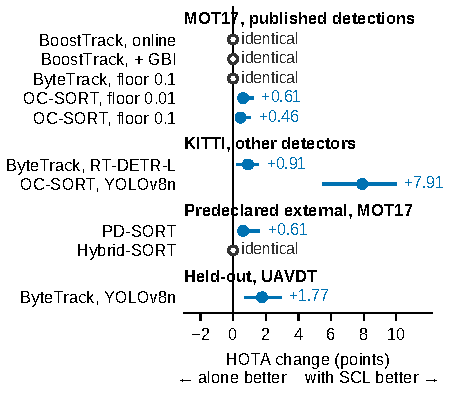
\includegraphics[width=0.62\textwidth]{figures/scl_forest_v3.pdf}
\caption{HOTA change with SCL (tracker with SCL minus tracker alone, in points) on MOT17, KITTI, and UAVDT. Dot and number: the change; line: its 95\% bootstrap interval; right of zero, SCL is better. Filled dot: a reliable gain; open dot: identical output.}
\label{fig:scl-forest}
\end{figure}

\subsection{MOT17 Evaluation Across Trackers}\label{sec:scl-res-mot17}
Table~\ref{tab:scl-mot17} shows the development trackers on MOT17 val-half. The two-stage trackers with well-matched detections kept the accuracy of their hosts: BoostTrack, online and with GBI, and ByteTrack at floor 0.1 gave exactly the same output through the self-limiting clean mode. The single-stage OC-SORT improved at both floors (HOTA from 66.43 to 67.04 and from 66.44 to 66.91, MOTA $+1.27$ and $+1.26$), with 8 fewer identity switches at floor 0.01 and higher HOTA on 7 of 7 sequences, through the continuation rescue.

\begin{table}[tbp]
\centering
\caption{MOT17 val-half, published YOLOX-X detections: each development tracker alone (Host) and with SCL (Host+SCL). Change: Host+SCL minus Host, with its 95\% paired-bootstrap interval (10,000 resamples, seed 42); bold: a reliable change. Paper: the value reported by the tracker's authors (--: not reported). Floor: the lowest emitted detector score. IDS: identity switches, a count (lower is better).}
\label{tab:scl-mot17}
\begin{tabular}{lrrrl}
\toprule
Metric & Paper & Host & Host+SCL & Change [95\% CI]\\
\midrule
\multicolumn{5}{l}{\textit{BoostTrack, online} \cite{stanojevic2024boosttrack}}\\
\quad HOTA & 68.37 & 68.49 & 68.49 & 0 (identical)\\
\quad MOTA & 75.56 & 75.50 & 75.50 & 0 (identical)\\
\quad IDF1 & 81.35 & 81.41 & 81.41 & 0 (identical)\\
\quad IDS & 118 & 113 & 113 & 0 (identical)\\
\multicolumn{5}{l}{\textit{BoostTrack, + GBI} \cite{stanojevic2024boosttrack}}\\
\quad HOTA & 71.33 & 71.73 & 71.73 & 0 (identical)\\
\quad MOTA & 80.55 & 81.03 & 81.03 & 0 (identical)\\
\quad IDF1 & 83.84 & 84.16 & 84.16 & 0 (identical)\\
\quad IDS & 106 & 97 & 97 & 0 (identical)\\
\multicolumn{5}{l}{\textit{ByteTrack, floor 0.1} \cite{zhang2022bytetrack}}\\
\quad HOTA & -- & 67.70 & 67.70 & 0 (identical)\\
\quad MOTA & 76.6 & 77.60 & 77.60 & 0 (identical)\\
\quad IDF1 & 79.3 & 79.47 & 79.47 & 0 (identical)\\
\quad IDS & -- & 214 & 214 & 0 (identical)\\
\multicolumn{5}{l}{\textit{OC-SORT, floor 0.01} \cite{cao2023ocsort}}\\
\quad HOTA & 66.5 & 66.43 & 67.04 & \textbf{$+0.61$ [$+0.36$, $+1.24$]}\\
\quad MOTA & 74.9 & 74.67 & 75.94 & \textbf{$+1.27$ [$+0.17$, $+3.01$]}\\
\quad IDS & -- & 211 & 203 & \textbf{$-8$ [$-15$, $-2$]}\\
\multicolumn{5}{l}{\textit{OC-SORT, floor 0.1} \cite{cao2023ocsort}}\\
\quad HOTA & 66.5 & 66.44 & 66.91 & \textbf{$+0.46$ [$+0.27$, $+1.09$]}\\
\quad MOTA & 74.9 & 74.67 & 75.93 & \textbf{$+1.26$ [$+0.37$, $+3.34$]}\\
\quad IDF1 & 77.7 & 78.05 & 78.33 & \textbf{$+0.287$ [$+0.003$, $+0.838$]}\\
\bottomrule
\end{tabular}
\end{table}

\subsection{KITTI Evaluation with Other Detectors}\label{sec:scl-res-kitti}
Table~\ref{tab:scl-kitti} shows what happens when the detector is replaced. With the noisy RT-DETR-L, SCL raised ByteTrack by 5.98 MOTA, 3.87 IDF1, and 0.91 HOTA points and BoT-SORT by 7.86 MOTA and 3.10 IDF1 points, with 297 and 226 fewer identity switches. With YOLOv8n, OC-SORT rose from 36.27 to 44.18 HOTA ($+7.91$ points, [$+5.47$, $+9.98$]), 9.40 MOTA points, and 9.60 IDF1 points, as its missed objects (FN) fell by 5,310. Figure~\ref{fig:scl-example} follows this cell over three frames: each object keeps its ID, and at frame 102 OC-SORT alone tracked 6 of the 10 labelled objects and with SCL 9.

\begin{table}[tbp]
\centering
\caption{KITTI tracking training with detectors the trackers were not tuned for (official HOTA, averaged over cars and pedestrians); columns as in Table~\ref{tab:scl-mot17}. BoT-SORT leaves out sequence 0020 in both runs, because its code stops with a numerical error on it; the other 20 sequences are used.}
\label{tab:scl-kitti}
\begin{tabular}{lrrl}
\toprule
Metric & Host & Host+SCL & Change [95\% CI]\\
\midrule
\multicolumn{4}{l}{\textit{ByteTrack} \cite{zhang2022bytetrack}\textit{, RT-DETR-L}}\\
\quad HOTA & 50.73 & 51.64 & \textbf{$+0.91$ [$+0.22$, $+1.55$]}\\
\quad MOTA & 47.27 & 53.24 & \textbf{$+5.98$ [$+1.16$, $+9.94$]}\\
\quad IDF1 & 64.98 & 68.86 & \textbf{$+3.87$ [$+1.67$, $+5.06$]}\\
\quad IDS & 686 & 389 & \textbf{$-297$ [$-530$, $-122$]}\\
\multicolumn{4}{l}{\textit{BoT-SORT} \cite{aharon2022botsort}\textit{, RT-DETR-L} (20 sequences)}\\
\quad MOTA & 48.25 & 56.11 & \textbf{$+7.86$ [$+2.21$, $+13.44$]}\\
\quad IDF1 & 67.74 & 70.85 & \textbf{$+3.10$ [$+1.00$, $+4.57$]}\\
\quad IDS & 476 & 250 & \textbf{$-226$ [$-369$, $-120$]}\\
\multicolumn{4}{l}{\textit{OC-SORT} \cite{cao2023ocsort}\textit{, YOLOv8n}}\\
\quad HOTA & 36.27 & 44.18 & \textbf{$+7.91$ [$+5.47$, $+9.98$]}\\
\quad MOTA & 33.99 & 43.39 & \textbf{$+9.40$ [$+1.10$, $+12.30$]}\\
\quad IDF1 & 50.46 & 60.05 & \textbf{$+9.60$ [$+5.61$, $+12.16$]}\\
\bottomrule
\end{tabular}
\end{table}

\begin{figure}[tbp]
\centering
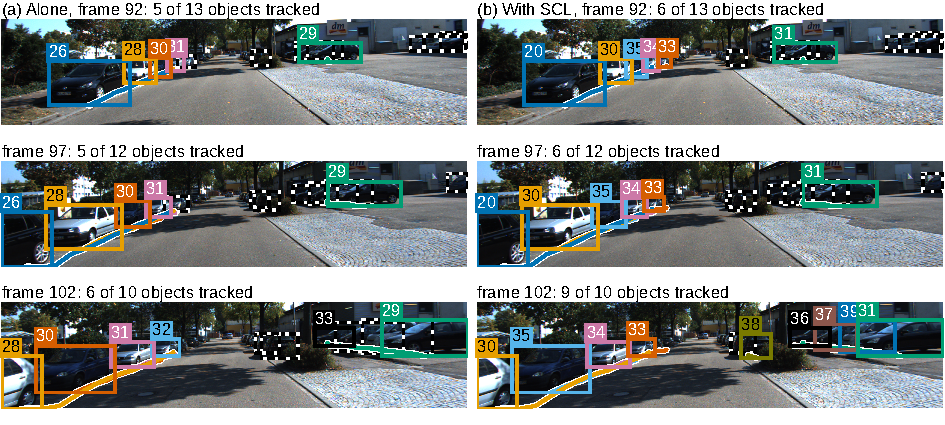
\includegraphics[width=0.98\textwidth]{figures/scl_kitti_example_v3.pdf}
\caption{KITTI sequence 0001 \cite{geiger2012kitti} tracked by OC-SORT with YOLOv8n at frames 92, 97, and 102 (rows): (a) the tracker alone; (b) with SCL. Each colour and number is one track; its line shows the object's last 20 frames. Dashed boxes: labelled objects that no track follows. IDs are numbered separately in each run. The sequence has the median HOTA gain of the 21 sequences, and frame 102 is its first frame with the largest gain in tracked objects.}
\label{fig:scl-example}
\end{figure}

\subsection{Evaluation under Shifted Detector Scores}\label{sec:scl-res-shift}
Table~\ref{tab:scl-shift} shows the trackers under the score transforms. Halving the scores reduced ByteTrack (official setting) and OC-SORT to 0 HOTA; with the layer they reached 66.17 and 66.72. Cubing reduced them to 60.92 and 58.34, and the layer restored them to 65.81 and 66.60; BoostTrack rose from 61.33 to 64.84. With $T=2$, the layer raised ByteTrack and OC-SORT by 1.11 and 1.24 points. Across the score changes, the layer raised HOTA significantly in 7 conditions.

\begin{table}[tbp]
\centering
\caption{MOT17 val-half with the detector scores changed before the tracker, which keeps its published thresholds: $s^3$ cubes every score, $0.5\,s$ halves it, and $T=2$ divides its logit by 2. HOTA (\%) of the tracker alone (Host) and with SCL (Host+SCL); 0.00: no object tracked; Change with its 95\% paired-bootstrap interval; bold: a reliable change. Lowest emitted score 0.01 (BoostTrack 0.1).}
\label{tab:scl-shift}
\begin{tabular}{lrrl}
\toprule
Score change & Host & Host+SCL & Change [95\% CI]\\
\midrule
\multicolumn{4}{l}{\textit{ByteTrack, official setting} \cite{zhang2022bytetrack}}\\
\quad $s^3$ & 60.92 & 65.81 & \textbf{$+4.89$ [$+2.60$, $+13.69$]}\\
\quad $0.5\,s$ & 0.00 & 66.17 & \textbf{$+66.17$ [$+49.32$, $+75.40$]}\\
\quad $T=2$ & 65.84 & 66.95 & \textbf{$+1.11$ [$+0.35$, $+3.87$]}\\
\multicolumn{4}{l}{\textit{OC-SORT} \cite{cao2023ocsort}}\\
\quad $s^3$ & 58.34 & 66.60 & \textbf{$+8.26$ [$+5.86$, $+16.81$]}\\
\quad $0.5\,s$ & 0.00 & 66.72 & \textbf{$+66.72$ [$+50.32$, $+75.56$]}\\
\quad $T=2$ & 65.99 & 67.22 & \textbf{$+1.24$ [$+0.52$, $+3.42$]}\\
\multicolumn{4}{l}{\textit{BoostTrack, online} \cite{stanojevic2024boosttrack}}\\
\quad $s^3$ & 61.33 & 64.84 & \textbf{$+3.51$ [$+0.85$, $+13.28$]}\\
\quad $T=2$ & 67.59 & 67.59 & 0 (identical)\\
\bottomrule
\end{tabular}
\end{table}

\subsection{Frozen Evaluation on External Trackers}\label{sec:scl-res-external}
Table~\ref{tab:scl-external} gives the two predeclared external systems. PD-SORT \cite{wang2025pdsort} was reproduced exactly; with SCL, its HOTA rose from 68.01 to 68.62 ($+0.61$ points, [$+0.27$, $+1.65$]), its MOTA by 1.13 ([$+0.27$, $+3.03$]), and its IDF1 by 0.82 ([$+0.43$, $+1.94$]), with higher HOTA on 7 of 7 sequences. Like OC-SORT, it is a single-stage tracker, but it was not seen during design. Hybrid-SORT \cite{yang2024hybridsort}, a two-stage tracker, gave identical output, as predicted before the run.

\begin{table}[tbp]
\centering
\caption{The two external trackers, chosen before the run and not used during design (MOT17 val-half, the authors' detections), each run once with the frozen SCL; columns as in Table~\ref{tab:scl-mot17}. Paper: the authors' number (for PD-SORT, their released output). EXACT: Host within 0.2 HOTA of it; CLOSE: within 1.0.}
\label{tab:scl-external}
\begin{tabular}{lrrrl}
\toprule
Metric & Paper & Host & Host+SCL & Change [95\% CI]\\
\midrule
\multicolumn{5}{l}{\textit{PD-SORT} \cite{wang2025pdsort}\textit{, EXACT}}\\
\quad HOTA & 68.01 & 68.01 & 68.62 & \textbf{$+0.61$ [$+0.27$, $+1.65$]}\\
\quad MOTA & 75.19 & 75.19 & 76.31 & \textbf{$+1.13$ [$+0.27$, $+3.03$]}\\
\quad IDF1 & 81.03 & 81.03 & 81.85 & \textbf{$+0.82$ [$+0.43$, $+1.94$]}\\
\multicolumn{5}{l}{\textit{Hybrid-SORT} \cite{yang2024hybridsort}\textit{, CLOSE}}\\
\quad HOTA & 67.1 & 66.70 & 66.70 & 0 (identical)\\
\quad MOTA & 75.8 & 75.52 & 75.52 & 0 (identical)\\
\quad IDF1 & 78.0 & 77.56 & 77.56 & 0 (identical)\\
\quad IDS & -- & 259 & 259 & 0 (identical)\\
\bottomrule
\end{tabular}
\end{table}

\subsection{Held-Out UAVDT Evaluation}\label{sec:scl-res-uavdt}
On the held-out UAVDT test split (Table~\ref{tab:scl-uavdt}), SCL raised the HOTA of the YOLOv8n stream from 29.05 to 30.83 ($+1.77$ points, [$+0.70$, $+2.94$]) and its IDF1 by 3.97 points, and cut identity switches by 45\%. With RT-DETR-L, whose host produced many false positives (MOTA 3.29), SCL raised MOTA from 3.29 to 27.99 ($+24.70$ points, [$+10.06$, $+51.08$]) and IDF1 by 5.74 points, and cut false positives by 58\% and identity switches by 56\%.

\begin{table}[tbp]
\centering
\caption{The held-out UAVDT test split (20 drone videos, not used during design), run once with the frozen SCL and ByteTrack with its published setting; columns as in Table~\ref{tab:scl-kitti}.}
\label{tab:scl-uavdt}
\begin{tabular}{lrrl}
\toprule
Metric & Host & Host+SCL & Change [95\% CI]\\
\midrule
\multicolumn{4}{l}{\textit{ByteTrack, RT-DETR-L} \cite{zhang2022bytetrack,zhao2024rtdetr}}\\
\quad MOTA & 3.29 & 27.99 & \textbf{$+24.70$ [$+10.06$, $+51.08$]}\\
\quad IDF1 & 48.59 & 54.33 & \textbf{$+5.74$ [$+0.13$, $+13.11$]}\\
\quad IDS & 1041 & 455 & \textbf{$-586$ [$-951$, $-248$]}\\
\multicolumn{4}{l}{\textit{ByteTrack, YOLOv8n} \cite{zhang2022bytetrack,jocher2023yolov8}}\\
\quad HOTA & 29.05 & 30.83 & \textbf{$+1.77$ [$+0.70$, $+2.94$]}\\
\quad IDF1 & 34.52 & 38.49 & \textbf{$+3.97$ [$+1.88$, $+6.17$]}\\
\quad IDS & 719 & 393 & \textbf{$-326$ [$-691$, $-73$]}\\
\bottomrule
\end{tabular}
\end{table}

\section{Comparison with Adaptive-Threshold Methods}\label{sec:scl-compare}
SCL adapts the thresholds of the tracker, so its gains must be compared with methods that adapt the thresholds alone. This section compares it with two simple adaptive baselines built from the same Otsu splits and with ACT, the closest published method (Section~\ref{sec:rw-thresholds}).

\subsection{Comparison with Adaptive-Threshold Baselines}\label{sec:scl-baselines}
Two simple baselines set the tracker's matching and birth thresholds in every frame to the first or second Otsu split of the logits of the last 10 frames, $t_1$ or $t_2$, and pass the scores unchanged. On KITTI (Table~\ref{tab:scl-baselines}), SCL reached the highest HOTA in all three cells, 2.2 to 8.6 points above the baselines, with intervals against the $t_2$ baseline above zero in every cell, so adaptive thresholds alone do not explain the gains.

\begin{table}[tbp]
\centering
\caption{KITTI tracking training: HOTA of the tracker alone (Host), of two adaptive baselines that set the tracker's thresholds in every frame to the first ($t_1$) or second ($t_2$) Otsu split of the logits of the last 10 frames, and of SCL. Halved: halved detector scores. SCL $-$ $t_2$: the gain over the stronger baseline, with its 95\% paired-bootstrap interval; bold: a reliable gain.}
\label{tab:scl-baselines}
\small\setlength{\tabcolsep}{4pt}
\begin{tabular}{lrrrrl}
\toprule
Cell & Host & $t_1$ & $t_2$ & SCL & SCL $-$ $t_2$ [95\% CI]\\
\midrule
OC-SORT, YOLOv8n & 36.27 & 39.97 & 41.09 & 44.18 & \textbf{$+3.09$ [$+2.00$, $+4.03$]}\\
ByteTrack, RT-DETR-L, halved & 49.50 & 49.58 & 49.50 & 51.79 & \textbf{$+2.29$ [$+0.28$, $+4.96$]}\\
OC-SORT, YOLOv8n, halved & 0.00 & 37.68 & 43.56 & 46.30 & \textbf{$+2.74$ [$+1.32$, $+3.34$]}\\
\bottomrule
\end{tabular}
\end{table}

\emph{Logit-to-score conversion.} The splits are found on logits and converted to scores with the logistic function; the thresholds recorded in every frame equalled the intended values, $\sigma(t_1)$ or $\sigma(t_2)$ in all eight baseline runs, and $\min(a,\sigma(t_2))$ (Eq.~\eqref{eq:scl-clean}) or 0.5 in the four KITTI cells of SCL, so every method received the thresholds it was meant to have.

\subsection{Comparison with ACT}\label{sec:scl-act}
ACT \cite{act2026adaptive}, the closest published method, sets ByteTrack's high and low thresholds in every frame from the first quartile and the number of the current scores, choosing between preset levels. It was run with its published parameters, without retuning, on the same detections and hosts as SCL (Tables~\ref{tab:scl-act} and~\ref{tab:scl-act-uavdt}): its high threshold became the host's matching threshold (with OC-SORT, its single threshold) and its low threshold the lower bound of the second step. With the host's own thresholds, the ACT runner reproduced the host exactly in all 84 KITTI and 40 UAVDT sequence runs. SCL reached significantly higher HOTA than ACT in every row of Table~\ref{tab:scl-act}: $+2.01$ and $+10.06$ points under halved scores and $+1.82$ with YOLOv8n on UAVDT. On UAVDT with RT-DETR-L (Table~\ref{tab:scl-act-uavdt}), SCL reached a MOTA of 27.99 against 5.34 for ACT ($+22.65$, [$+9.03$, $+47.21$]) and had 418 fewer identity switches, because the fixed score levels of ACT removed few of the host's false positives (178,219 against 78,975).

\begin{table}[tbp]
\centering
\caption{ACT \cite{act2026adaptive}, with its published parameters, and SCL on the same detections and tracker: HOTA with each method, and SCL $-$ ACT with its 95\% paired-bootstrap interval; bold: a reliable difference. KITTI: official HOTA, averaged over cars and pedestrians; UAVDT: test split.}
\label{tab:scl-act}
\begin{tabular}{lllrrl}
\toprule
Data & Detector & Tracker & ACT & SCL & SCL $-$ ACT [95\% CI]\\
\midrule
KITTI, halved & RT-DETR-L & ByteTrack & 49.77 & 51.79 & \textbf{$+2.01$ [$+0.01$, $+4.76$]}\\
KITTI, halved & YOLOv8n & OC-SORT & 36.24 & 46.30 & \textbf{$+10.06$ [$+6.88$, $+12.01$]}\\
UAVDT test & YOLOv8n & ByteTrack & 29.01 & 30.83 & \textbf{$+1.82$ [$+0.65$, $+3.00$]}\\
\bottomrule
\end{tabular}
\end{table}

\begin{table}[tbp]
\centering
\caption{MOTA and identity switches of ACT and SCL on the UAVDT test split with ByteTrack and RT-DETR-L. A positive MOTA difference and a negative IDS difference favour SCL; bold: a reliable difference.}
\label{tab:scl-act-uavdt}
\begin{tabular}{lrrl}
\toprule
Metric & ACT & SCL & SCL $-$ ACT [95\% CI]\\
\midrule
MOTA & 5.34 & 27.99 & \textbf{$+22.65$ [$+9.03$, $+47.21$]}\\
IDS & 873 & 455 & \textbf{$-418$ [$-718$, $-123$]}\\
\bottomrule
\end{tabular}
\end{table}

\section{Component Ablation and Parameter Sensitivity}\label{sec:scl-ablation}
Table~\ref{tab:scl-parts} removes one part of the frozen SCL, or changes one of its values, at a time on the three KITTI cells of Table~\ref{tab:scl-baselines}. Each part matters where its step acts. Without the weak detection recovery, the single-stage OC-SORT lost up to 3.35 HOTA points, as it has no low-score step of its own; without the noisy mode (always clean), the halved-score cells lost up to 2.44 points, without the remap up to 1.67, and without the motion tolerance up to 0.14. The clean mode, in turn, keeps well-matched trackers at their own accuracy (Table~\ref{tab:scl-prior}).

The sensitivity analysis, planned before the runs, changed the window $W$, the frames whose median decides the mode, the IoU of the duplicate and recovery rules, and the motion history. For every value and cell, HOTA stayed within 0.62 points of the frozen SCL, and within 0.24 points on a fourth cell, ByteTrack with the original RT-DETR-L scores. None of the values thus needs tuning for these detectors and trackers.

\begin{table}[tbp]
\centering
\caption{What each part and each fixed value of SCL contributes on the three KITTI cells of Table~\ref{tab:scl-baselines} (HOTA): (a) OC-SORT, YOLOv8n; (b) ByteTrack, RT-DETR-L, halved scores; (c) OC-SORT, YOLOv8n, halved scores. Upper part: one part removed at a time, with the largest HOTA loss and its cell. Lower part: one fixed value changed at a time (frozen value in brackets), with the largest HOTA change over the tested values and cells. Frozen SCL, HOTA: (a) 44.18, (b) 51.79, (c) 46.30.}
\label{tab:scl-parts}
\begin{tabular}{lrl}
\toprule
Part removed & Largest loss & Cell\\
\midrule
Weak detection recovery & 3.35 & (a)\\
Noisy mode (always clean) & 2.44 & (c)\\
Remap (raw scores) & 1.67 & (b)\\
Motion tolerance & 0.14 & (c)\\
\midrule
Value changed (frozen) & Largest change & Tested\\
\midrule
Window $W$ (10 frames) & 0.56 & 5, 20\\
Mode median frames (all) & 0.36 & last 100, 300\\
Duplicate/recovery IoU (0.5) & 0.62 & 0.4, 0.6\\
Motion history (100 frames) & 0.09 & 50, 200\\
\bottomrule
\end{tabular}
\end{table}

\section{Runtime}\label{sec:scl-runtime}
SCL needs no training, no GPU, and no access to the inside of the detector or the tracker. On the processor of Table~\ref{tab:scl-setup} it takes 2.95 ms per frame, small next to the 42 ms of the detector, and the tracker itself ran faster with it (1.43 against 2.04 ms per frame); the end-to-end time rose by only 4.5\%. A new tracker is added through its four published contract values and an adapter, without changes to the rules.

\section{Discussion}\label{sec:scl-discussion}
\emph{The score scale is part of the MOT system.} Halving the scores reduced ByteTrack and OC-SORT from 67.70 and 66.43 HOTA to 0, and with RT-DETR-L on UAVDT ByteTrack reached a MOTA of only 3.29. A tracker's fixed thresholds hold only for the detector they were tuned for, so the score scale deserves the same attention as the association method. SCL treats the compatibility between a detector's score scale and a tracker's thresholds as a property that can be checked and restored online, which answers RQ2 for the tested trackers and detectors.

\emph{Selective by design.} In the clean mode SCL keeps the tracker's thresholds and scores, so a well-matched tracker receives its normal input: BoostTrack, ByteTrack at floor 0.1, and Hybrid-SORT gave exactly the output of their hosts. This is the main difference from the earlier design AOB, which acted in every frame and lowered the HOTA of the same strong trackers by 4.15 to 5.89 points (Table~\ref{tab:scl-prior}). The layer therefore does not need to know in advance whether a tracker needs help; it reads the answer from the scores.

\emph{Host-aware adaptation.} Single-stage trackers gained mainly through the continuation rescue, which gives them the step that two-stage trackers already have: OC-SORT and PD-SORT, a tracker not seen during design, on MOT17, and OC-SORT with YOLOv8n on KITTI, where removing the rescue cost up to 3.35 HOTA points (Table~\ref{tab:scl-parts}). Two-stage trackers gained when the detector was noisy or its scores shifted, as ByteTrack and BoT-SORT with RT-DETR-L. The same frozen rules served both kinds of tracker through their published contract values.

\emph{Wide applicability.} One frozen configuration served seven trackers of both kinds, four detection sources, and three datasets of people and vehicles filmed from the ground, from a car, and from drones (RQ3). The splits move exactly with a stretch or shift of the logits, and the layer also restored the trackers under cubed scores (Section~\ref{sec:scl-res-shift}), so it follows the common ways in which a detector's score scale changes.

\emph{Deployment.} The layer runs on an ordinary processor in a few milliseconds per frame (Section~\ref{sec:scl-runtime}), and a new tracker is added through its four published contract values and an adapter, without changes to the rules. The label-free mode and the confident share $\rho$ can also be logged as a running check that a new or retrained detector still fits its tracker.

\emph{Scope of the evaluation.} The layer was evaluated with tracking-by-detection trackers that expose published score thresholds, on MOT17, KITTI, and UAVDT, with the detection sources of Table~\ref{tab:scl-setup}, and its runtime was measured on one processor. Trackers that learn detection and association jointly keep their thresholds inside the network and are outside the scope of the host contract; extending the layer to them is a direction for future work (Section~\ref{sec:conc-future}). SCL does not choose the detector operating point, which is the task of AC-MOT.

\section{Summary}\label{sec:scl-summary}
This chapter treated the compatibility between a detector's score scale and a tracker's thresholds as a property that can be checked and restored online, without labels and without changing either component. SCL checks it with nested Otsu splits of recent logits and a whole-stream majority rule, leaves compatible pairs as they are, and restores incompatible ones through the tracker's own published settings, with a track-guided recovery of weak detections that gives single-stage trackers the continuation step they lack. The layer was developed step by step from an earlier always-on design and frozen before any external test. The frozen layer was tested on seven trackers and four detection sources. Under halved scores, it restored two trackers from 0 to about 66 HOTA; with a mismatched detector on held-out aerial data, it raised MOTA by up to 24.70 points; well-matched trackers kept their own accuracy; it reached higher HOTA than simple adaptive thresholds and than the published ACT method; and it took 2.95 ms per frame on average on a CPU. Detector--tracker compatibility can therefore be managed as part of the tracking system, so a detector can be replaced or retrained without retuning the tracker. The next chapter draws the conclusions of the thesis as a whole.
